El método de reducción aquí presentado, es una adaptación del propuesto por Abdolhosseinzadeh \citep{Abdolhosseinzadeh2015}. El cual consiste en reducir el óxido de grafeno incorporando una solución acuosa de ácido ascórbico.
\\
Como precursor se utiliza el óxido de grafeno producto del método previamente descrito y como agente reductor se emplea ácido ascórbico (\ce{C_6H_8O_6}, Sigma-Aldrich $>$95\%). Se disuelven 30 g de ácido ascórbico en 300 ml de agua destilada, que es agregado al óxido de grafeno obtenido bajo agitación (aproximadamente 300 ml en dispersión acuosa). En este procedimiento, la mezcla gradualmente se torna negra, siendo ésta una señal de que la reducción se está llevando a cabo. Además, la mezcla se vuelve una dispersión heterogénea, signo de la hidrofobicidad del óxido reducido de grafeno (rGO). La mezcla es llevada a 90 \degree C y se mantiene por 1 hr dentro del rango de temperatura entre 85 y 95 \degree C. Posteriormente, el compuesto se deja decantar y es lavado cinco veces con 1 l de agua destilada. De este modo se obtiene una dispersión de óxido reducido de grafeno con agua como medio dispersante.

\section{Resultados}
En la figura \ref{fig:RGOyGO} se muestran dispersiones en medio acuoso de los productos de la síntesis antes descrita.
Los materiales obtenidos son caracterizados por espectroscopia de rayos x (XRD), Raman y microcopia SEM.

\begin{figure}[h]
	\centering
	\begin{subfigure}{0.4\textwidth}
		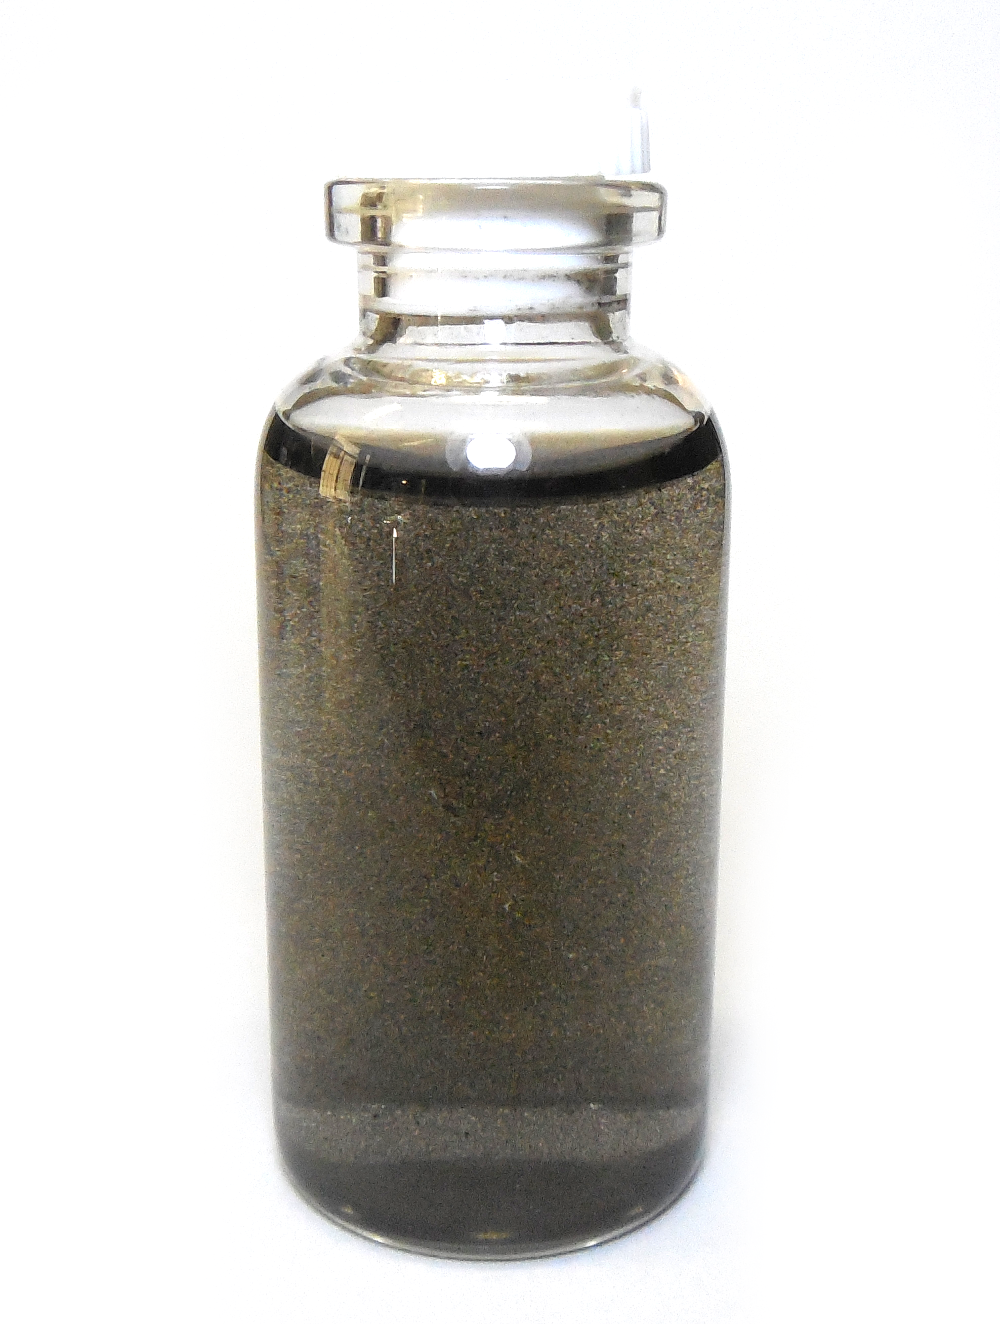
\includegraphics[width=\textwidth]{RGO_pic.png}
		\caption{rGO}
		\label{fig:RGO}
	\end{subfigure}
	\begin{subfigure}{0.42\textwidth}
		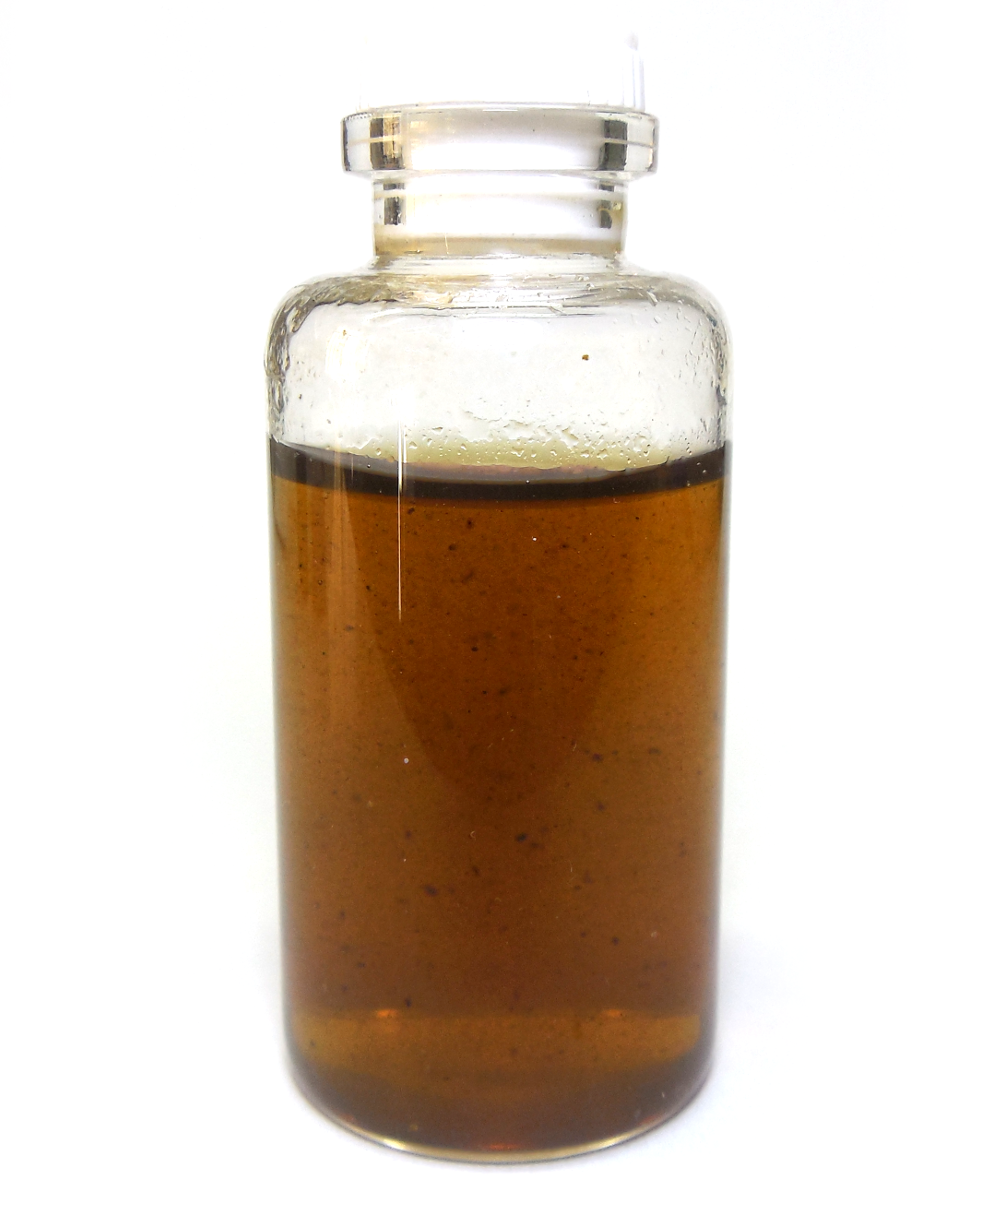
\includegraphics[width=\textwidth]{GO_pic.png}
		\caption{GO}
		\label{fig:GO}
	\end{subfigure}
	\caption{Dispersiones de rGO y GO en agua.}
	\label{fig:RGOyGO}
\end{figure}

En la figura \ref{fig:xrd} se presenta un gráfico del espectro de difracción de rayos x para las muestras sintetizadas de grafito, GO y rGO, obtenido en un difractómetro de rayos X Shimazdu XRD 6000, con radiación Cu $K\alpha_1$ y $K\alpha_2$ ($\lambda$ = 1,5418 \AA{} ). El pico principal en el espectro del grafito se encuentra en 26,2\degree, lo que corresponde a una distancia interplanar de 0,34 nm. El óxido de grafeno presenta un pico principal en 10,2\degree, que corresponde a una distancia interplanar de 0,87 nm. El óxido reducido de grafeno tienen un pico principal en 22,6\degree, correspondiente a una distancia interplanar de 0,39 nm. Esto indica que el grafito al oxidarse, efectivamente aumenta su distancia interplanar considerablemente debido a la incorporación de grupos oxigenados. Al reducir el óxido de grafeno y remover estos grupos funcionales, la distancia interplanar disminuye, acercándose a la del grafito, pero sin alcanzar el valor original del grafito, pues la reducción no es completa\citep{Guo2009, Marcano2010, Park2011, Li2014, Stobinski2014, Xu2014a, Yang2014, Abdolhosseinzadeh2015}.

%\begin{figure}[h]
%	\centering
%	\begin{tikzpicture}[]
%		\begin{axis}[
%			cycle list name=colorbrewer-RYB,
%			no markers,
%			width = \textwidth,
%			yticklabels={,,},
%			ylabel={Intensidad [u.a.]},
%			xlabel={2 $\theta$ [grados]},
%			legend entries={Grafito, Óxido de grafeno, Óxido de grafeno reducido}]
%			\addplot table [x expr = \thisrow{2t}, y expr=\thisrow{C}] {./Data/XRD/xrd.txt};
%			\addplot table [x expr = \thisrow{2t}, y expr=\thisrow{GO}+1] {./Data/XRD/xrd.txt};
%			\pgfplotsset{cycle list shift=1}
%			\addplot table [x expr = \thisrow{2t}, y expr=\thisrow{RGO}+2] {./Data/XRD/xrd.txt};
%%			\addplot table [x expr = \thisrow{2t}, y expr=\thisrow{RGOLYO}+3] {./Data/XRD/xrd.txt};
%			\addplot +[mark=none, solid, black] coordinates {(10, 0) (10, 3)};
%			\addplot +[mark=none, solid, black] coordinates {(23, 0) (23, 3)};
%			\addplot +[mark=none, solid, black] coordinates {(26, 0) (26, 3)};
%			\node[black, left] at (10, 3){\small{10\degree}};
%			\node[black, left] at (23, 3){\small{23\degree}};
%			\node[black, right] at (26, 3){\small{26\degree}};
%		\end{axis}
%	\end{tikzpicture}
%	\caption{Espectro de difracción de rayos x.}
%	\label{fig:xrd}
%\end{figure}
\begin{figure}[h]
	\centering
	\begin{tikzpicture}[]
	\begin{axis}[
	cycle list name=colorbrewer-RYB,
	no markers,
	width = \textwidth,
	yticklabels={,,},
	ylabel={Intensidad [u.a.]},
	xlabel={2 $\theta$ [grados]},
	legend entries={Grafito, Óxido de grafeno, Óxido de grafeno reducido}]
	\addplot table [x expr = \thisrow{2t}, y expr=\thisrow{C}] {./Data/XRD/xrd.txt};
	\addplot table [x expr = \thisrow{2t}, y expr=\thisrow{GO}+1] {./Data/XRD/xrd.txt};
	\pgfplotsset{cycle list shift=1}
	\addplot table [x expr = \thisrow{2t}, y expr=\thisrow{RGO}+2] {./Data/XRD/xrd.txt};
%	\addplot table [x expr = \thisrow{2t}, y expr=\thisrow{RGOLYO}+3] {./Data/XRD/xrd.txt};
	\node[black, rotate=90] at (24, 0.3){\small{(002)}};
%	\node[black, rotate=90] at (7, 1.5){\small{10,2\degree}};
%	\node[black, rotate=90] at (26, 3){\small{22,6\degree}};
	\end{axis}
	\end{tikzpicture}
	\caption{Espectro de difracción de rayos x.}
	\label{fig:xrd}
\end{figure}

\begin{figure}
	\centering
	\begin{tikzpicture}[]
		\begin{axis}[
		cycle list name=colorbrewer-RYB,
		no markers,
		width = \textwidth,
		ylabel={Intensidad [u.a.]},
		xlabel={$\mathrm{cm^{-1}}$},
		legend entries={Óxido de grafeno, Óxido de grafeno reducido}]
		\addplot+[restrict x to domain=1000:3500] table [x expr = \thisrow{raman_shift}, y expr=\thisrow{CRGO090615_1}] {./Data/RAMAN/raman.txt};
%		\addplot+[restrict x to domain=1000:3500] table [x expr = \thisrow{raman_shift}, y expr=\thisrow{GO090615_1} + 10] {./Data/RAMAN/raman.txt};
		\pgfplotsset{cycle list shift=1}
		\addplot+[restrict x to domain=1000:3500] table [x expr = \thisrow{raman_shift}, y expr=\thisrow{GO090615_2} + 20] {./Data/RAMAN/raman.txt};
		%	\addplot table [x expr = \thisrow{2t}, y expr=\thisrow{RGOLYO}+3] {./Data/XRD/xrd.txt};
		%	\node[black, rotate=90] at (7, 1.5){\small{10,2\degree}};
		%	\node[black, rotate=90] at (26, 3){\small{22,6\degree}};
		\end{axis}
	\end{tikzpicture}
	\caption{Raman.}
	\label{fig:raman}
\end{figure}

La imagen de la figura \ref{fig:rgo_paper_sem}, es una microscopia de barrido de un electrodo de rGO en forma de papel.

\begin{figure}
	\centering
	\begin{subfigure}{\textwidth}
		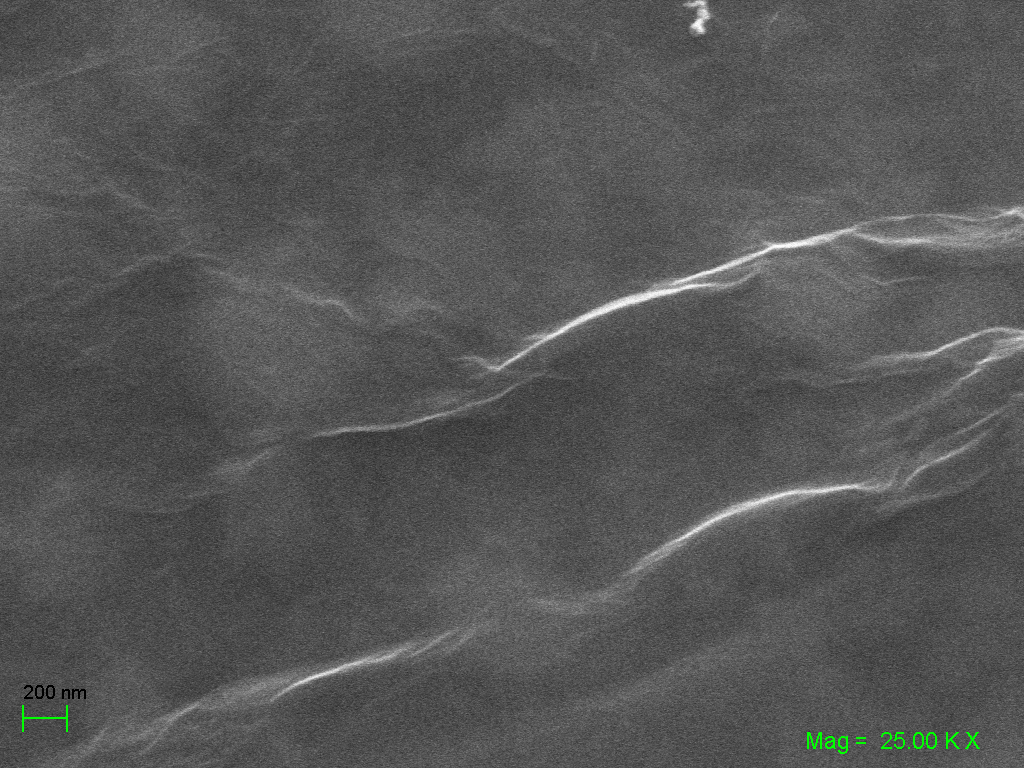
\includegraphics[width=\textwidth]{CRGO300517_paper.png}
	\end{subfigure}
	\begin{subfigure}{\textwidth}
		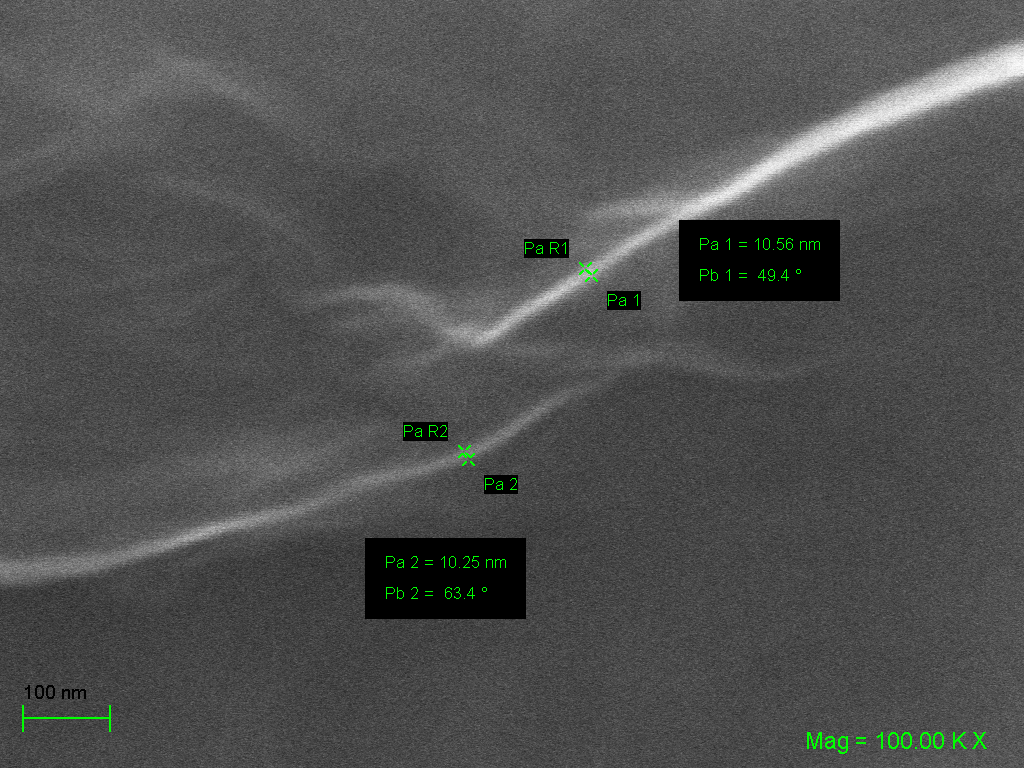
\includegraphics[width=\textwidth]{CRGO300517_paper_measures.png}
	\end{subfigure}
	\caption{Imagen SEM de la muestra \mPapelAcero.}
	\label{fig:rgo_paper_sem}
\end{figure}
